% Class talk (about 7 minutes). Build: make (slides PDF and speaker-notes PDF).
\documentclass[aspectratio=169,10pt]{beamer}
% shared preamble for the final presentation and the class talk
\usetheme[progressbar=frametitle,numbering=fraction]{metropolis}
\usepackage[T1]{fontenc}
\usepackage{booktabs,tabularx,array,xcolor,tikz,pgfpages,listings}
\usetikzlibrary{arrows.meta,positioning,fit,calc,shapes.geometric}
\definecolor{ink}{HTML}{17262B}\definecolor{acc}{HTML}{1F5FAD}\definecolor{ok}{HTML}{2E7D32}
\definecolor{warn}{HTML}{D9822B}\definecolor{pale}{HTML}{EEF3F8}
\setbeamercolor{frametitle}{bg=ink}
\setbeamercolor{progress bar}{fg=acc}
\setbeamercolor{alerted text}{fg=acc}
\setbeamertemplate{note page}[plain]
\usepackage{xspace}
\newcommand{\pg}{PostgreSQL\xspace}
\newcolumntype{L}[1]{>{\raggedright\arraybackslash}p{#1}}
\newcolumntype{Y}{>{\raggedright\arraybackslash}X}
\newcommand{\ok}[1]{\textcolor{ok}{\textbf{#1}}}
\newcommand{\wa}[1]{\textcolor{warn}{\textbf{#1}}}
\tikzset{
  box/.style={draw=acc,rounded corners=2pt,align=center,fill=pale,font=\scriptsize,minimum height=9mm,text width=22mm},
  io/.style={draw=gray,align=center,fill=gray!10,font=\scriptsize,minimum height=8mm,text width=19mm},
  orc/.style={draw=ok,rounded corners=2pt,align=center,fill=ok!8,font=\scriptsize,minimum height=7mm,text width=22mm},
  fl/.style={-{Stealth[length=1.6mm]},thick,draw=ink},
  bk/.style={-{Stealth[length=1.6mm]},dashed,draw=acc}}

\ifdefined\shownotes\setbeameroption{show only notes}\fi
\title{Grammar-Aware Fuzzing of PostgreSQL, and Beyond}
\subtitle{CS-5187 Software Analysis, Term Project A3}
\author{Venu Kummari \and Bhuvan Chilukuti \and Gowtham Reddy}
\institute{IIT Guwahati}
\date{November 2026}

\begin{document}

\maketitle
\note{VENU. Good afternoon. I am Venu, with Bhuvan and Gowtham. We built a fuzzer, a
dynamic-analysis tool that automatically generates test queries for PostgreSQL and decides by
itself whether an answer is wrong. It found nine PostgreSQL bugs; six are fixed upstream, five with
our patches. We then generalized it to four more SQL engines, where we filed three more fixes. We
focus on how the tool works and how it found the bugs.}

\begin{frame}{Problem: the oracle for wrong results}
\begin{columns}[T]
\column{0.52\textwidth}
\begin{itemize}
  \item Target: \pg, master built with \textbf{assertions}, compared with release 18.6.
  \item Four failure classes: crash/assertion, \textbf{wrong result}, internal error, hang.
  \item A wrong result leaves no trace: the tool needs a \alert{test oracle} that knows the right answer.
\end{itemize}
\column{0.44\textwidth}
\begin{block}{Idea}
Generate SQL as \alert{typed derivation trees}; rewrite each tree into
\alert{equivalent queries} and run it under \alert{other plans} and on the \alert{last
release}. Any disagreement is a bug.
\end{block}
\end{columns}
\end{frame}
\note{VENU. A fuzzer can run millions of queries; the hard part is to know that an answer is
wrong. Our answer is comparison: equivalent questions must give equal answers.}

\begin{frame}{Architecture of the \pg fuzzer}
\centering\resizebox{\linewidth}{!}{% architecture of the PostgreSQL fuzzer
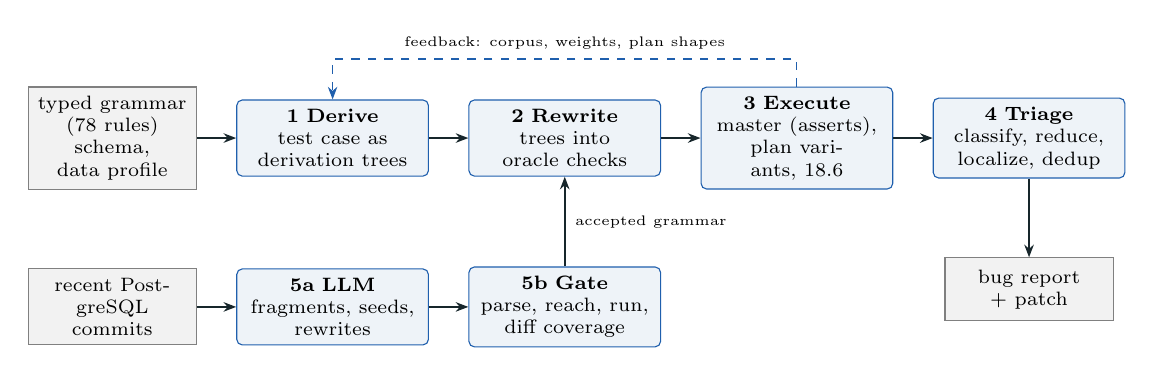
\begin{tikzpicture}[node distance=4mm and 5mm]
\node[io] (g) {typed grammar (78 rules)\\schema, data profile};
\node[box,right=of g] (s1) {\textbf{1 Derive}\\test case as\\derivation trees};
\node[box,right=of s1] (s2) {\textbf{2 Rewrite}\\trees into\\oracle checks};
\node[box,right=of s2] (s3) {\textbf{3 Execute}\\master (asserts),\\plan variants, 18.6};
\node[box,right=of s3] (s4) {\textbf{4 Triage}\\classify, reduce,\\localize, dedup};
\node[io,below=10mm of g] (c) {recent \pg commits};
\node[box,right=of c] (l1) {\textbf{5a LLM}\\fragments, seeds,\\rewrites};
\node[box,right=of l1] (l2) {\textbf{5b Gate}\\parse, reach, run,\\diff coverage};
\node[io,below=10mm of s4] (r) {bug report\\+ patch};
\draw[fl] (g)--(s1); \draw[fl] (s1)--(s2); \draw[fl] (s2)--(s3); \draw[fl] (s3)--(s4); \draw[fl] (s4)--(r);
\draw[bk] (s3.north) -- ++(0,0.35) -| node[pos=0.25,above,font=\tiny]{feedback: corpus, weights, plan shapes} (s1.north);
\draw[fl] (c)--(l1); \draw[fl] (l1)--(l2); \draw[fl] (l2.north) -- node[right,font=\tiny]{accepted grammar} (s2.south -| l2.north);
\end{tikzpicture}
}
\small
\begin{itemize}
  \item One derivation tree, four jobs: \alert{generate, mutate, rewrite into oracles, reduce}.
  \item 10{,}500 lines of Python, 151 unit tests.
\end{itemize}
\end{frame}
\note{VENU. Five steps. Derive a test case from our typed grammar; rewrite its trees into
oracle checks; execute on master, under other planner settings and on 18.6; triage the failures.
The LLM loop reads recent commits and proposes new grammar, which enters only if it passes a gate
on the real server.}

\begin{frame}{Techniques: grammar and oracles}
\small
\begin{columns}[T]
\column{0.42\textwidth}
\textbf{Typed grammar} (own DSL, 78 rules)
\begin{itemize}
  \item types as parameters, scope-aware names $\Rightarrow$ \alert{99.3\%} valid statements (random mutation 26\%)
  \item feedback: corpus, subtree mutation, bandit weights, data-aware literals
\end{itemize}
\column{0.55\textwidth}
\textbf{Oracle stack}
\begin{itemize}
  \item server watches: crash/assertion (server log), internal error \texttt{XX000}, hang (timeout and cancel ignored)
  \item \textbf{plan variants}: 18 planner settings, same answer required
  \item \textbf{metamorphic tree rewrites}: TLP $Q = Q_p \uplus Q_{\neg p} \uplus Q_{p\ \mathrm{IS\ NULL}}$, NoREC, $e \rightarrow (\mathrm{SELECT}\ e)$
  \item \textbf{cross-version}: master vs 18.6
  \item \textbf{CERT}: a restriction must not raise the row estimate
\end{itemize}
\end{columns}
\end{frame}
\note{GOWTHAM. The grammar carries SQL types, so generated queries are valid and reach the
planner. On top sits a stack of oracles. Three just watch the server. The others compare two
answers that must agree. Because we keep the tree, a rewrite is type-correct at any nesting level.}

\begin{frame}{Techniques: triage and the LLM gate}
\small
\begin{columns}[T]
\column{0.48\textwidth}
\textbf{Triage}
\begin{enumerate}
  \item reproduce $\times3$ on a fresh server
  \item reduce on the tree (smallest derivation of the same type), then statements, then tokens: 116 $\rightarrow$ 79 tokens
  \item localize: plan variant, rewrite or version
  \item deduplicate by signature
\end{enumerate}
\column{0.48\textwidth}
\textbf{LLM proposes, server decides}
\begin{itemize}
  \item reads a recent commit, proposes grammar, seeds, rewrites
  \item gate: parses, reachable, $\geq60\%$ runs, executes the commit's \alert{changed lines} (gcov)
  \item 4 of 10 commits passed
\end{itemize}
\end{columns}
\end{frame}
\note{BHUVAN. Triage makes a failure reportable: reproduce it, shrink it while keeping it valid by
replaying trees, and find which setting or rewrite flips it. The LLM is never trusted on its word:
PostgreSQL itself decides what enters the fuzzer.}

\begin{frame}{How the tool found the \pg bugs}
\scriptsize
\begin{tabularx}{\linewidth}{@{}L{0.18\linewidth}L{0.24\linewidth}YL{0.16\linewidth}@{}}
\toprule
Bug type & Found by & Signal & Upstream \\
\midrule
assertion & LLM fragment + TLP check & assertion during a metamorphic check & \ok{fixed} \#19803 \\
wrong output & cross-version oracle & master and 18.6 disagreed & \ok{fixed, our patch} \\
assertion & extended-statistics generator & assertion in the estimator & \ok{fixed, our patch} \\
assertion / wrong result & grammar fuzzer + cross-version & assertion on master, wrong answer on 18.6 & \ok{fixed, our patch} \\
wrong result & cross-version + TLP & extra row on master & \ok{fixed, our patch} \\
hang & hang oracle & timeout and cancel ignored & \ok{fixed, our patch} \\
internal error & \texttt{XX000} oracle & ``should not happen'' error & \wa{confirmed} \\
wrong result & $e\rightarrow(\mathrm{SELECT}\ e)$ rewrite & sub-select blocked a simplification & \wa{open} \\
bad estimate & CERT oracle & estimate rose under a restriction & \wa{open} \\
\bottomrule
\end{tabularx}

\smallskip
\small\textbf{9 reported, 6 fixed upstream (5 with our patches).} \texttt{scripts/reproduce.sh}: all 9 rediscovered in 150 s.
\end{frame}
\note{GOWTHAM and BHUVAN. Read the middle column: every oracle earned its place. Two bugs came
only from comparing versions, one only from the sub-select rewrite, one only from the hang
oracle, one only from the estimate oracle. After the oracle fired, triage reduced and localized
each case, and we wrote the root cause and the patch.}

\begin{frame}{Results}
\small
\begin{tabularx}{\linewidth}{@{}lY@{}}
\toprule
RQ1 reach & backend lines \textbf{36.7\% vs 22.2\%} for random mutation ($\hat A_{12}=1.00$, $p=0.008$); oracles: plan shapes $\times1.7$ \\
RQ2 precision & 93 candidates: 8 real, 15 duplicates, 42 false positives (all classes fixed), 28 flaky \\
RQ3 benchmark & 23 real bugs re-injected; best arm found 2 of 20 in 1 h \\
RQ4 LLM & +5 SQL features, no coverage gain \\
\bottomrule
\end{tabularx}

\medskip
Lesson: \alert{oracle precision}, not generator reach, limits a wrong-result fuzzer.
\end{frame}
\note{GOWTHAM. 5 trials of 1 hour per arm. Typing pays; oracles find real bugs, and their false
positives were the main cost.}

\begin{frame}{Beyond \pg: the generalized fuzzer}
\centering\resizebox{!}{0.6\textheight}{% architecture of the generalized fuzzer
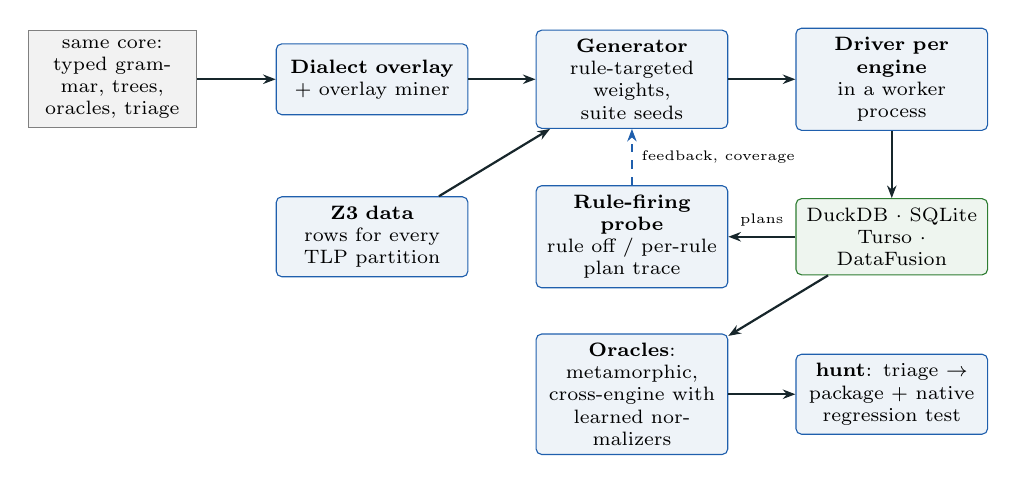
\begin{tikzpicture}
\node[io]  (core) at (0,0)     {same core: typed grammar, trees, oracles, triage};
\node[box] (ov)   at (3.3,0)   {\textbf{Dialect overlay}\\+ overlay miner};
\node[box] (gen)  at (6.6,0)   {\textbf{Generator}\\rule-targeted weights,\\suite seeds};
\node[box] (drv)  at (9.9,0)   {\textbf{Driver per engine}\\in a worker process};
\node[box] (z3)   at (3.3,-2)  {\textbf{Z3 data}\\rows for every\\TLP partition};
\node[box] (rule) at (6.6,-2)  {\textbf{Rule-firing probe}\\rule off / per-rule\\plan trace};
\node[orc] (eng)  at (9.9,-2)  {DuckDB $\cdot$ SQLite\\Turso $\cdot$ DataFusion};
\node[box] (orc)  at (6.6,-4)  {\textbf{Oracles}: metamorphic,\\cross-engine with\\learned normalizers};
\node[box] (hunt) at (9.9,-4)  {\textbf{hunt}: triage $\rightarrow$\\package + native\\regression test};
\draw[fl] (core)--(ov); \draw[fl] (ov)--(gen); \draw[fl] (gen)--(drv); \draw[fl] (drv)--(eng);
\draw[fl] (z3)--(gen);
\draw[fl] (eng)--node[above,font=\tiny]{plans}(rule);
\draw[bk] (rule)--node[right,font=\tiny]{feedback, coverage}(gen);
\draw[fl] (eng)--(orc); \draw[fl] (orc)--(hunt);
\end{tikzpicture}
}
\small
\begin{itemize}
  \item DuckDB, SQLite, Turso, DataFusion; same trees, oracles and triage.
\end{itemize}
\end{frame}
\note{VENU. We then made the tool target-independent. Each engine gets a driver in its own worker
process and a dialect overlay on the same grammar.}

\begin{frame}{Generalized techniques}
\small
\begin{itemize}
  \item \textbf{Dialect overlays} + \textbf{overlay miner}: failing grammar alternatives become \texttt{\%drop} lines (DuckDB 32\% $\rightarrow$ 44\% valid with no manual line; with overlays 79--98\% valid).
  \item \textbf{Optimizer-rule firing} instead of code coverage: a rule fires if the plan changes when it is switched off (SQLite test control, DuckDB \texttt{disabled\_optimizers}, DataFusion \texttt{EXPLAIN VERBOSE}); used as feedback, coverage and for \alert{rule-targeted generation}.
  \item \textbf{Z3 data synthesis}: rows that make every TLP partition non-empty.
  \item \textbf{Learned normalizers} for cross-engine comparison: disagreements 28.7\% $\rightarrow$ 3.6\%.
  \item \textbf{Autonomous loop}: campaign $\rightarrow$ triage $\rightarrow$ package with a regression test in the engine's own format.
\end{itemize}
\end{frame}
\note{BHUVAN. Rule firing works on release builds of any engine and is about the optimizer, where
logic bugs live. Normalizers make two engines comparable without hand-written rules.}

\begin{frame}{How the generalized fuzzer found its bugs}
\small
\begin{tabularx}{\linewidth}{@{}lL{0.2\linewidth}YL{0.22\linewidth}@{}}
\toprule
Engine & Bug type & Found by & State \\
\midrule
Turso & wrong result & Turso-vs-SQLite differential oracle & \wa{filed with fix}: \#11594 / PR \#11595 \\
DuckDB & internal error (regression) & internal-error oracle on the nightly build & \wa{filed with fix}: \#28551 / PR \#28552 \\
DataFusion & internal error in DML & internal-error oracle & \wa{filed with fix}: \#27235 / PR \#27236 \\
3 more & panic, errors & worker caught a panic / error & fixed upstream before we filed \\
\bottomrule
\end{tabularx}

\medskip
Each fix has a regression test in the engine's format and passes the engine's full suite.
\end{frame}
\note{VENU. Same pipeline as for PostgreSQL. The three pull requests were filed on 8 November and
await review.}

\begin{frame}{Conclusion}
\begin{columns}[T]
\column{0.32\textwidth}\centering{\Huge\textbf{9}}\\\small \pg bugs reported
\column{0.32\textwidth}\centering{\Huge\ok{6}}\\\small fixed upstream (5 our patches)
\column{0.32\textwidth}\centering{\Huge\textbf{3}}\\\small fixes filed to DuckDB, Turso, DataFusion
\end{columns}
\bigskip
\small Team: Venu (tool, paper, generalized fuzzer) $\cdot$ Bhuvan (RQ3, bug hunts, four patches) $\cdot$ Gowtham (campaigns, LLM arm, two reports, one fix).
\end{frame}
\note{GOWTHAM. Valid SQL is the easy part; knowing the right answer is the hard part. Thank you.}

\begin{frame}[standout]
Thank you. Questions?\\[6pt]
\normalsize github.com/PASS-IITG/cs5187-term-project-blazing-bhuvi
\end{frame}

\end{document}
